\section{Khảo sát có kiểm soát các bộ lọc và phân ngưỡng tạo ứng viên}
\label{sec:thuc_nghiem_loc_nguong}

\subsection{Thiết kế thí nghiệm sàng lọc 110 cấu hình trên tập Validation}

Chất lượng của tập vùng ứng viên ban đầu quyết định trần độ thu hồi của toàn hệ thống: nếu bộ lọc không đủ mạnh, nhiễu đốm sẽ sinh ra hàng vạn mảnh vụn nhỏ; ngược lại, nếu làm mượt quá mức, các dải dầu hẹp sẽ bị xóa nhòa. Để lựa chọn cấu hình tối ưu, nghiên cứu thực hiện khảo sát tích Descartes gồm \textbf{11 bộ lọc không gian} (\texttt{none}; \texttt{median} kích thước $\{3, 5\}$; \texttt{gaussian} $\sigma \in \{0.8, 1.2\}$; \texttt{lee} kích thước $\{3, 5, 7\} \times L \in \{1, 4\}$) và \textbf{10 bộ phân ngưỡng} (\texttt{otsu} toàn cục; \texttt{niblack} cục bộ với cửa sổ $\{15, 31, 51\} \times k \in \{0.2, 0.5, 0.8\}$), tạo thành $110$ tổ hợp chạy trên toàn bộ $671$ ảnh Validation (cố định $A_{\min} = 16$).

\begin{figure}[!htbp]
\centering
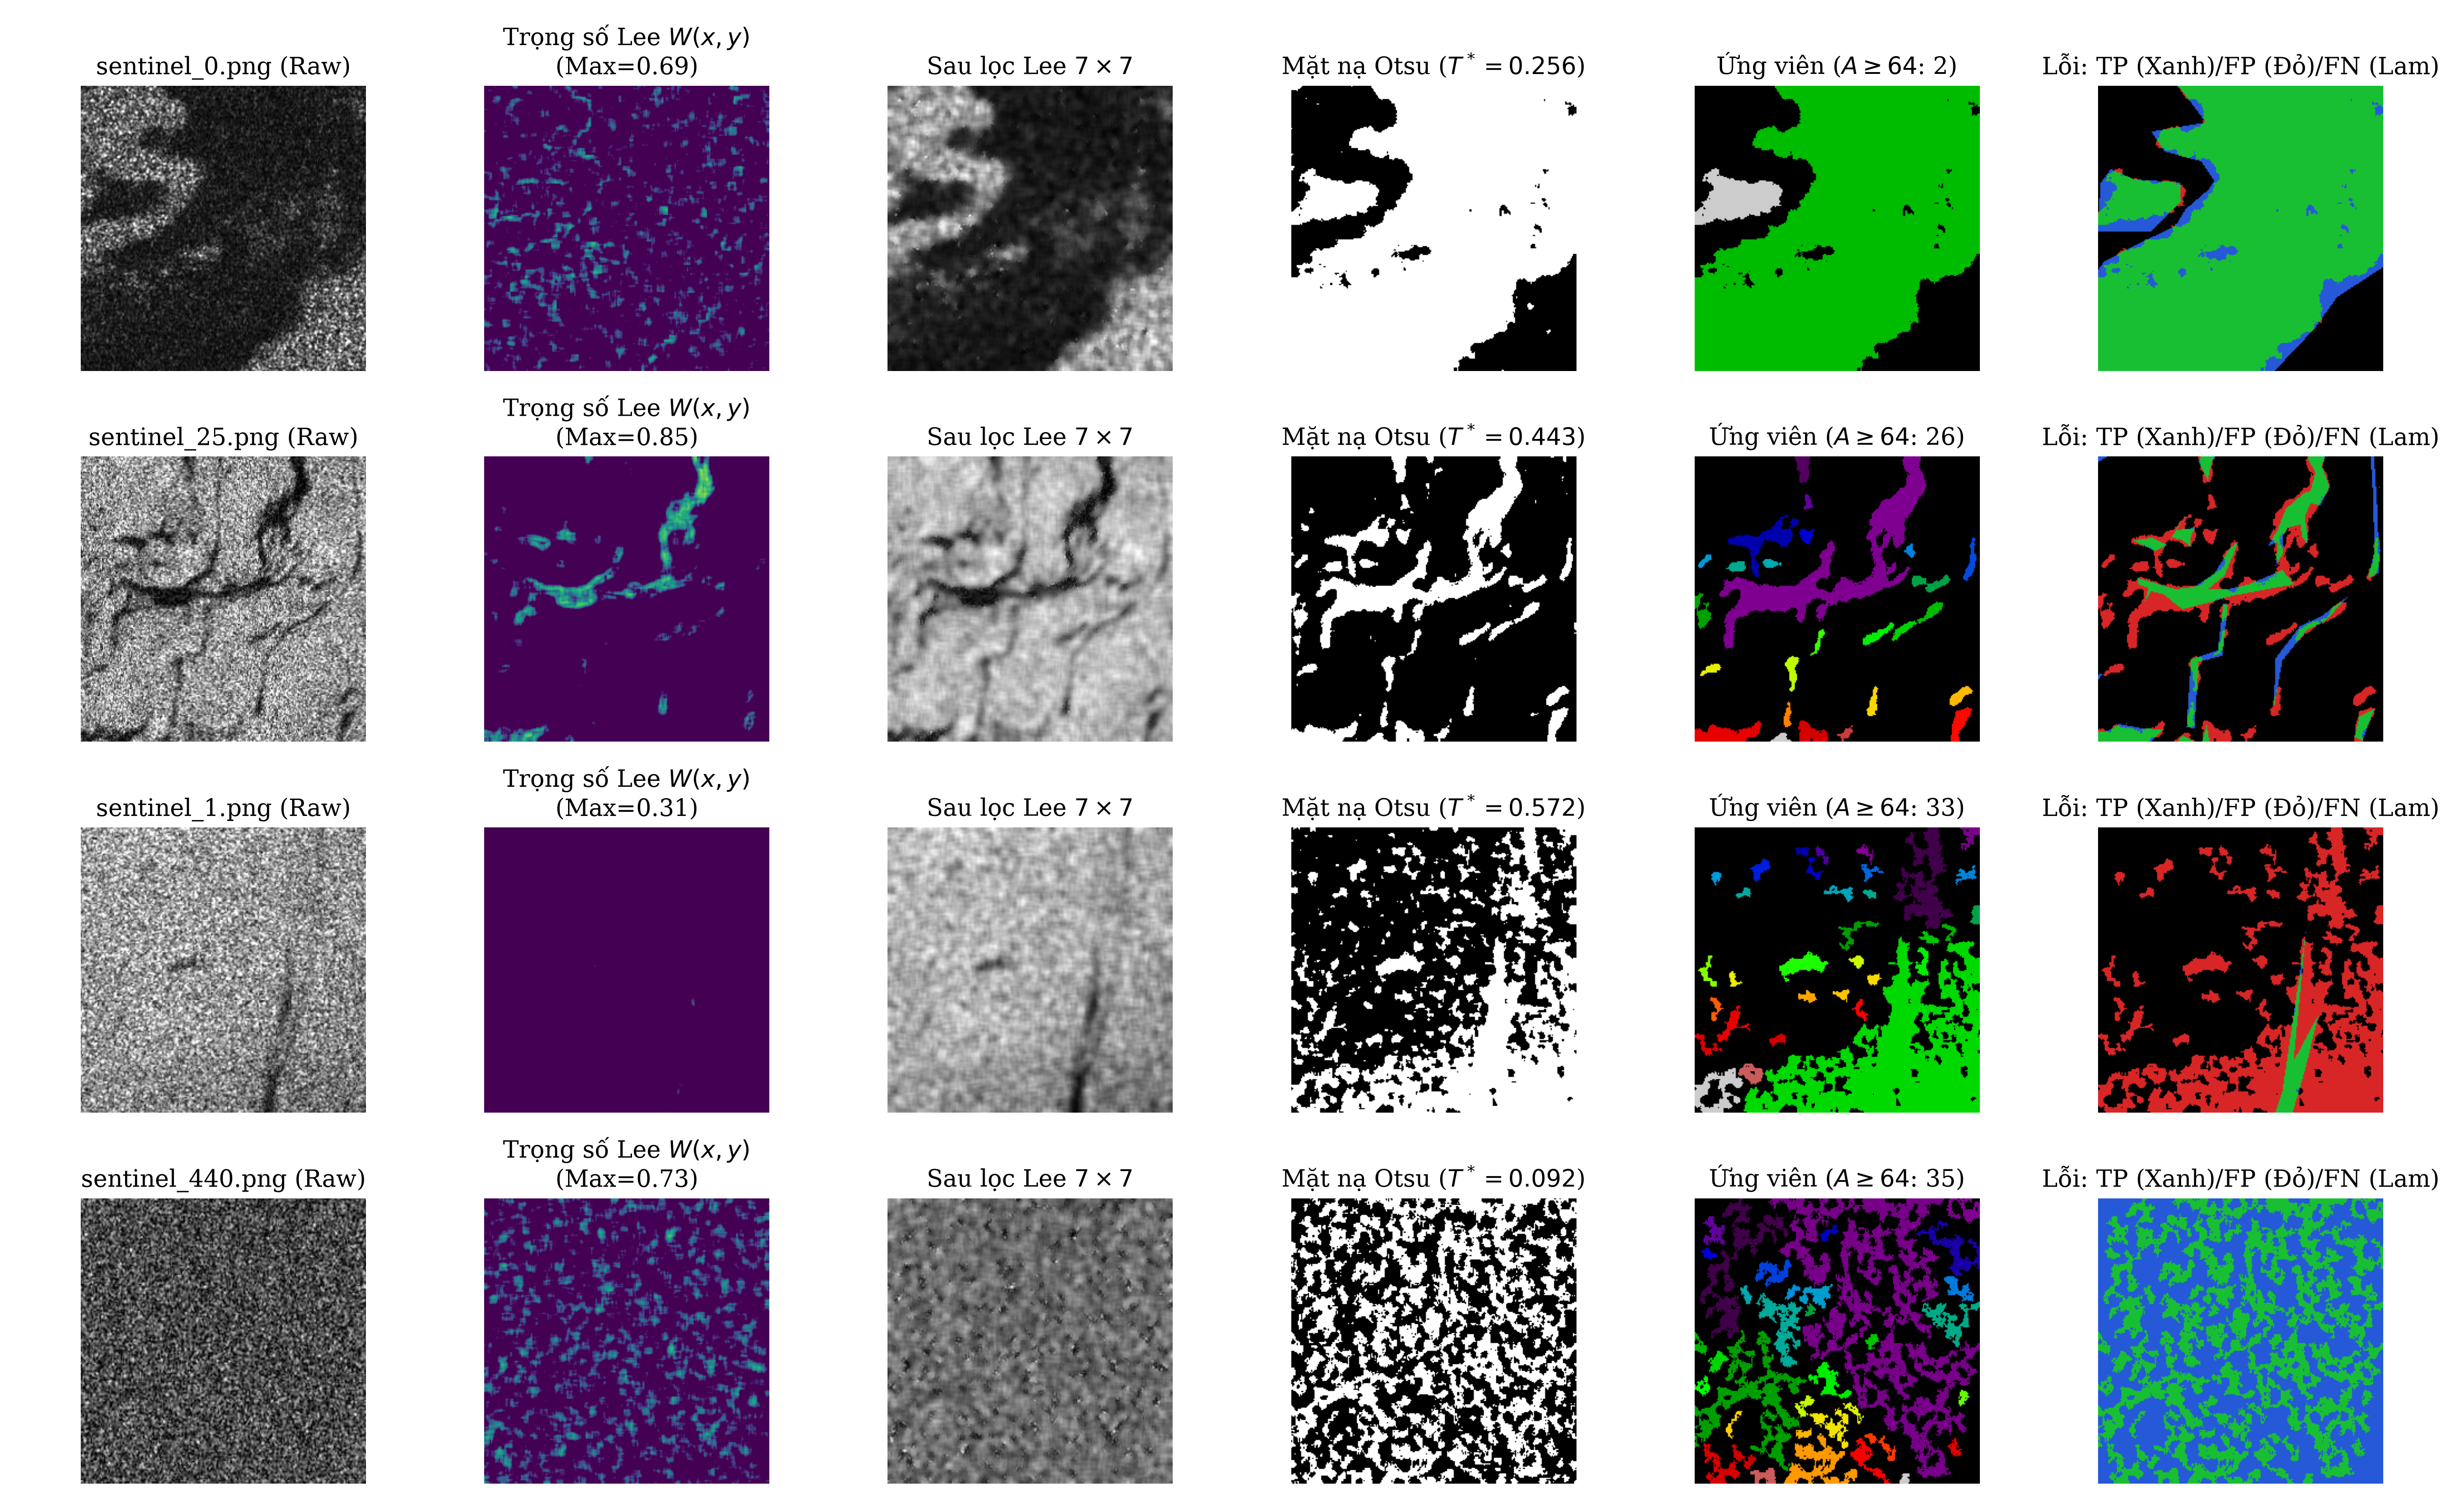
\includegraphics[width=\textwidth]{figures/fig3_step_by_step_pipeline.png}
\caption{Trực quan hóa các bước biến đổi trung gian của quy trình trên 4 cảnh SAR đại diện: Ảnh gốc $\to$ Bản đồ trọng số Lee $W(x, y)$ $\to$ Ảnh sau lọc Lee $7 \times 7$ $\to$ Mặt nạ nhị phân Otsu $\to$ Vùng ứng viên sau lọc diện tích $\ge 64$ $\to$ Bản đồ phân loại lỗi điểm ảnh (Xanh lá: TP, Đỏ: FP, Lam: FN).}
\label{fig:step_by_step_pipeline}
\end{figure}

Hình~\ref{fig:step_by_step_pipeline} trực quan hóa các bước trung gian của quy trình. Bảng~\ref{tab:filter_benchmark} tổng hợp kết quả định lượng chi tiết của 13 cấu hình lọc không gian tiêu biểu kết hợp với phân ngưỡng Otsu, kèm khoảng tin cậy Bootstrap 95\% của mức chênh lệch $\Delta\text{F1}$ tính qua $2\,000$ lần lấy mẫu lại có hoàn lại.

\begin{table}[!htbp]
\centering
\small
\caption{So sánh có kiểm soát 13 cấu hình lọc không gian (cố định phân ngưỡng Otsu, $A_{\min} = 16$) trên 671 ảnh Validation. Khoảng tin cậy Bootstrap 95\% của $\Delta\text{F1}$ so với Lee $7 \times 7$ ($L=4$).}
\label{tab:filter_benchmark}
\resizebox{\textwidth}{!}{%
\begin{tabular}{|l|c|c|c|c|c|c|c|c|}
\hline
\textbf{Cấu hình bộ lọc} & \textbf{TP} & \textbf{FP} & \textbf{FN} & \textbf{Prec} & \textbf{Rec} & \textbf{Cand F1} & \textbf{Pix IoU} & \textbf{$\Delta\text{F1}$ vs. Lee $7\times 7, L=4$ (95\% CI)} \\ \hline
\textit{None (Không lọc)} & 518 & $39\,283$ & $2\,222$ & 0.0130 & 0.1891 & 0.0244 & 0.4272 & $+0.0612 \quad [+0.0534, +0.0693]$ \\ \hline
\textit{Median $3 \times 3$} & 758 & $50\,479$ & $1\,982$ & 0.0148 & 0.2766 & 0.0281 & 0.4780 & $+0.0574 \quad [+0.0508, +0.0645]$ \\ \hline
\textit{Median $5 \times 5$} & 910 & $36\,046$ & $1\,830$ & 0.0246 & 0.3321 & 0.0458 & 0.5241 & $+0.0397 \quad [+0.0346, +0.0451]$ \\ \hline
\textit{Gaussian $\sigma = 0.8$} & 794 & $47\,039$ & $1\,946$ & 0.0166 & 0.2898 & 0.0314 & 0.4849 & $+0.0541 \quad [+0.0476, +0.0608]$ \\ \hline
\textit{Gaussian $\sigma = 1.2$} & 895 & $40\,877$ & $1\,845$ & 0.0214 & 0.3266 & 0.0402 & 0.5118 & $+0.0453 \quad [+0.0398, +0.0513]$ \\ \hline
\textit{Lee $3 \times 3$ ($L=1$)} & 821 & $46\,341$ & $1\,919$ & 0.0174 & 0.2996 & 0.0329 & 0.4909 & $+0.0526 \quad [+0.0462, +0.0592]$ \\ \hline
\textit{Lee $3 \times 3$ ($L=4$)} & 822 & $46\,897$ & $1\,918$ & 0.0172 & 0.3000 & 0.0326 & 0.4907 & $+0.0529 \quad [+0.0466, +0.0595]$ \\ \hline
\textit{Lee $5 \times 5$ ($L=1$)} & 961 & $32\,247$ & $1\,779$ & 0.0289 & 0.3507 & 0.0535 & 0.5365 & $+0.0321 \quad [+0.0278, +0.0367]$ \\ \hline
\textit{Lee $5 \times 5$ ($L=4$)} & 967 & $32\,486$ & $1\,773$ & 0.0289 & 0.3529 & 0.0534 & 0.5355 & $+0.0321 \quad [+0.0281, +0.0366]$ \\ \hline
\textit{Lee $7 \times 7$ ($L=1$)} & $1\,034$ & $20\,770$ & $1\,706$ & 0.0474 & 0.3774 & 0.0843 & 0.5645 & $+0.0013 \quad [-0.0004, +0.0031]$ \\ \hline
\textbf{Lee $7 \times 7$ ($L=4$) [Chọn]} & $\mathbf{1\,049}$ & $\mathbf{20\,743}$ & $\mathbf{1\,691}$ & \textbf{0.0481} & \textbf{0.3828} & \textbf{0.0855} & \textbf{0.5629} & \textbf{Mốc tham chiếu chuẩn} \\ \hline
\textit{Mean $7 \times 7$ [Đối chứng]} & $1\,033$ & $20\,787$ & $1\,707$ & 0.0473 & 0.3770 & 0.0841 & 0.5646 & $+0.0014 \quad [-0.0003, +0.0033]$ \\ \hline
\textit{Median $7 \times 7$ [Đối chứng]} & 999 & $22\,856$ & $1\,741$ & 0.0419 & 0.3646 & 0.0751 & 0.5557 & $+0.0104 \quad [+0.0075, +0.0134]$ \\ \hline
\end{tabular}%
}
\end{table}

\begin{figure}[!htbp]
\centering
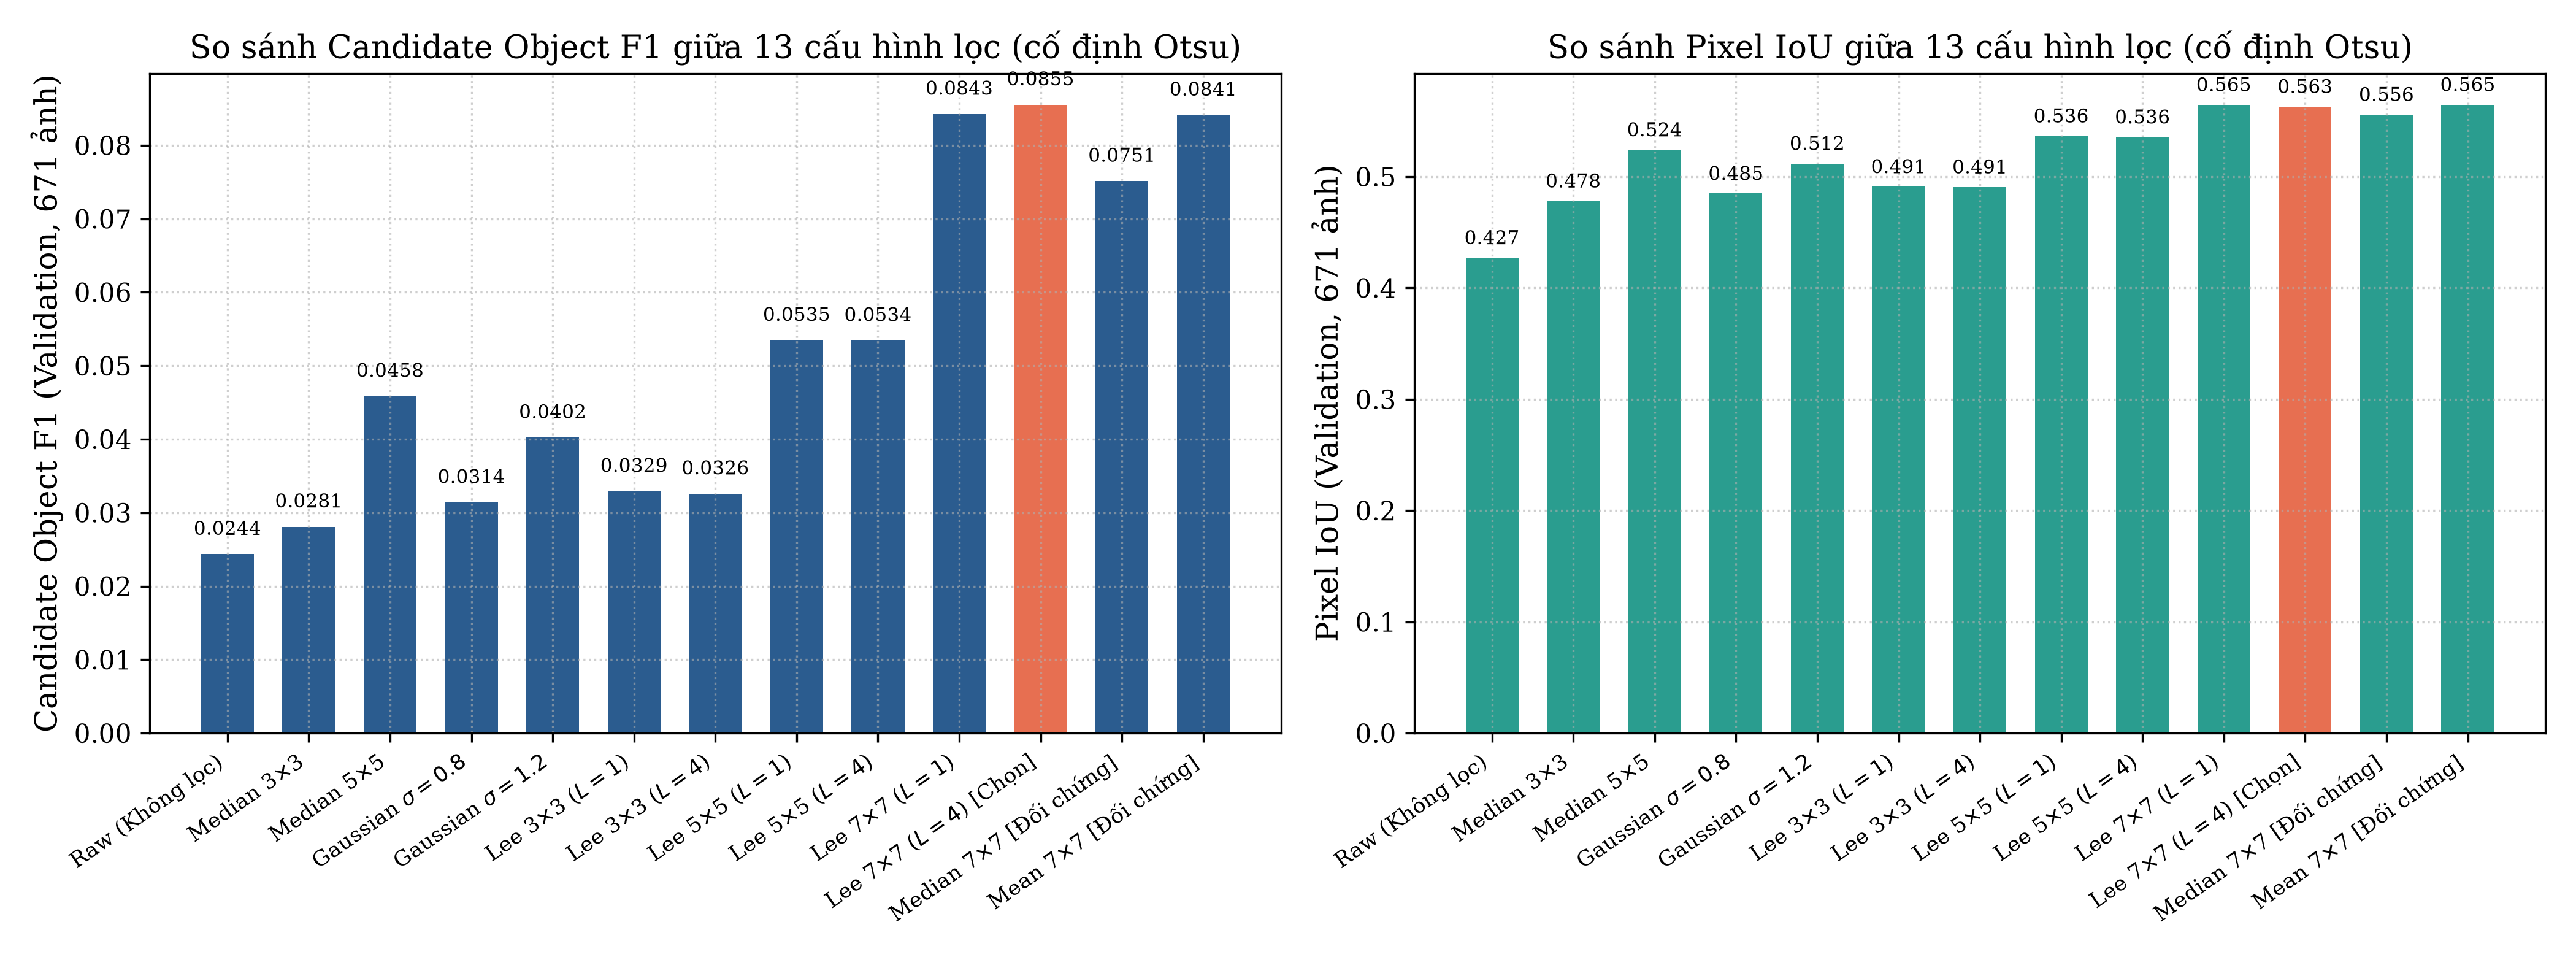
\includegraphics[width=0.96\textwidth]{figures/fig4_filter_threshold_benchmark.png}
\caption{Đối sánh định lượng Candidate Object F1 và Pixel IoU giữa 13 cấu hình lọc không gian (cố định Otsu, $A_{\min}=16$) trên 671 ảnh Validation.}
\label{fig:filter_benchmark_plot}
\end{figure}

\subsection{Phân tích thực nghiệm và hiện tượng suy biến của bộ lọc Lee trên ảnh 8-bit}

Từ Bảng~\ref{tab:filter_benchmark} và Hình~\ref{fig:filter_benchmark_plot}, kết quả thực nghiệm cho thấy 3 phát hiện chính:

\begin{enumerate}
    \item \textbf{Hiệu quả giảm báo nhầm khi mở rộng cửa sổ lọc:}
    Trong dải kích thước cửa sổ $\{3 \times 3, 5 \times 5, 7 \times 7\}$, việc tăng kích thước lên $7 \times 7$ giúp cắt giảm hơn $55\%$ số lượng mảnh nhiễu báo nhầm (từ $>46\,000$ FP xuống còn $\approx 20\,700$ FP), đồng thời nâng Candidate F1 đơn điệu từ $0.0326$ ($3 \times 3$) lên $0.0534$ ($5 \times 5$) và đạt đỉnh $0.0855$ ($7 \times 7$).

    \item \textbf{Hiện tượng suy biến của trọng số Lee về bộ lọc trung bình hộp (mean filter):}
    Cấu hình Lee $7 \times 7$ ($L=4$, F1 $= 0.0855$) đạt chỉ số cao nhất trong không gian quét ban đầu. Tuy nhiên, khi bổ sung phép đối chứng có kiểm soát với bộ lọc trung bình hộp Mean $7 \times 7$ (F1 $= 0.0841$), độ chênh lệch $\Delta\text{F1} = +0.0014$ có khoảng tin cậy Bootstrap 95\% $[-0.0003, +0.0033]$ chứa giá trị 0 (không có ý nghĩa thống kê).
    
    \textit{Giải thích cơ chế:} Do ảnh PNG trong bộ dữ liệu SOS đã qua tiền xử lý làm mượt sơ bộ bởi nhà phát hành, số looks hiệu dụng thực tế trên các vùng biển đồng nhất ($\text{ENL}_{\text{eff}} = m^2 / v$) lớn hơn rất nhiều so với tham số giả định $L \in \{1, 4\}$. Hệ quả là điều kiện $v(x, y) \le m(x, y)^2/L$ xảy ra trên hầu hết các điểm ảnh, khiến trọng số $W(x, y) = 0$ trên diện rộng (như ở hàng 3 Hình~\ref{fig:step_by_step_pipeline} với $\max W = 0.00$) và bộ lọc Lee suy biến về phép lấy trung bình hộp.

    \item \textbf{Sự suy giảm hiệu năng của phân ngưỡng cục bộ Niblack trên biển đồng nhất:}
    Toàn bộ 9 cấu hình Niblack đều ghi nhận hiệu năng thấp (F1 dao động từ $0.0013$ đến $0.0325$, số lượng báo nhầm tăng từ $40\,000$ đến hơn $154\,000$ FP). Nguyên nhân là ở các vùng biển lặng gió có độ biến thiên mức xám rất thấp ($s_W \approx 0$), ngưỡng động $T = m_W - k s_W$ bị hạ thấp và kích hoạt các điểm ảnh ở đuôi phân phối nhiễu thành các đốm tối giả mạo. Vì vậy, phân ngưỡng toàn cục Otsu là giải pháp phù hợp hơn cho bước tạo ứng viên.
\end{enumerate}
